\chapter{提案手法}
\label{method}
本章では提案手法の詳細を述べる.本研究はヘルメットをキーの代わりとして用いることを目標とし,圧力センサを搭載したヘルメットを装着して装着者の頭部形状を取得することで,個人識別を行う手法を提案する.\par
システム構成を図\ref{system}に示す.学習データ群および新たにプロトタイプデバイスから得られるデータは,32個のセンサ値であり32次元のベクトルとして扱う.提案するシステムではあらかじめ学習フェーズとして,所有者の頭部データを複数回収集しておく.このデータ群に対し,プロトタイプデバイスから得られたセンサ値のベクトルからのマハラノビス距離を計算する.マハラノビス距離とは統計学で用いられる一種の距離である.これは多次元のデータに対しても使用できる.データは32次元の連続ベクトルであり,学習フェーズで得られた多変数ベクトルのデータ列を
\[
  x^m = x_1, x_2, \ldots, x_m
\]
とすると,i番目のデータは
\[
  x_i = \left(
        \begin{array}{c}
            x_{i,1} \\
            x_{i,2} \\
            \vdots \\
            x_{i,32}
        \end{array}
    \right)
\]
と表すことができる.この平均値ベクトル$\mu$と分散共分散行列$\Sigma$は以下のように求められる.
\begin{eqnarray*}
  \mu &=& \frac{1}{m}\sum_{i=1}^{m}x_i \\
  \Sigma &=& \frac{1}{m}\sum_{i=1}^{m}(x_i-\mu)(x_i-\mu)^T
\end{eqnarray*}
このとき,学習データ群$x^m$に対する未知のユーザの入力データ$y$のマハラノビス距離は
\[
  D_{Mahalanobis} = \sqrt{(y-\mu)^{T}\Sigma^{-1}(y-\mu)}
\]
と定義される.ここで閾値を$\theta$と置き,
\[
  \theta < \sqrt{(y-\mu)^{T}\Sigma^{-1}(y-\mu)}
\]
を満たす場合,入力データ$y$は所有者以外の他人から得られた頭部データであると判定し異常値だとして拒否する.一方で,入力データ$y$に対して,
\[
  \theta \geq \sqrt{(y-\mu)^{T}\Sigma^{-1}(y-\mu)}
\]
を満たす場合,入力データ$y$は所有者本人から得られた頭部データであると判定し正常値だとして認証する.

\begin{figure}[!t]
  \begin{center}
    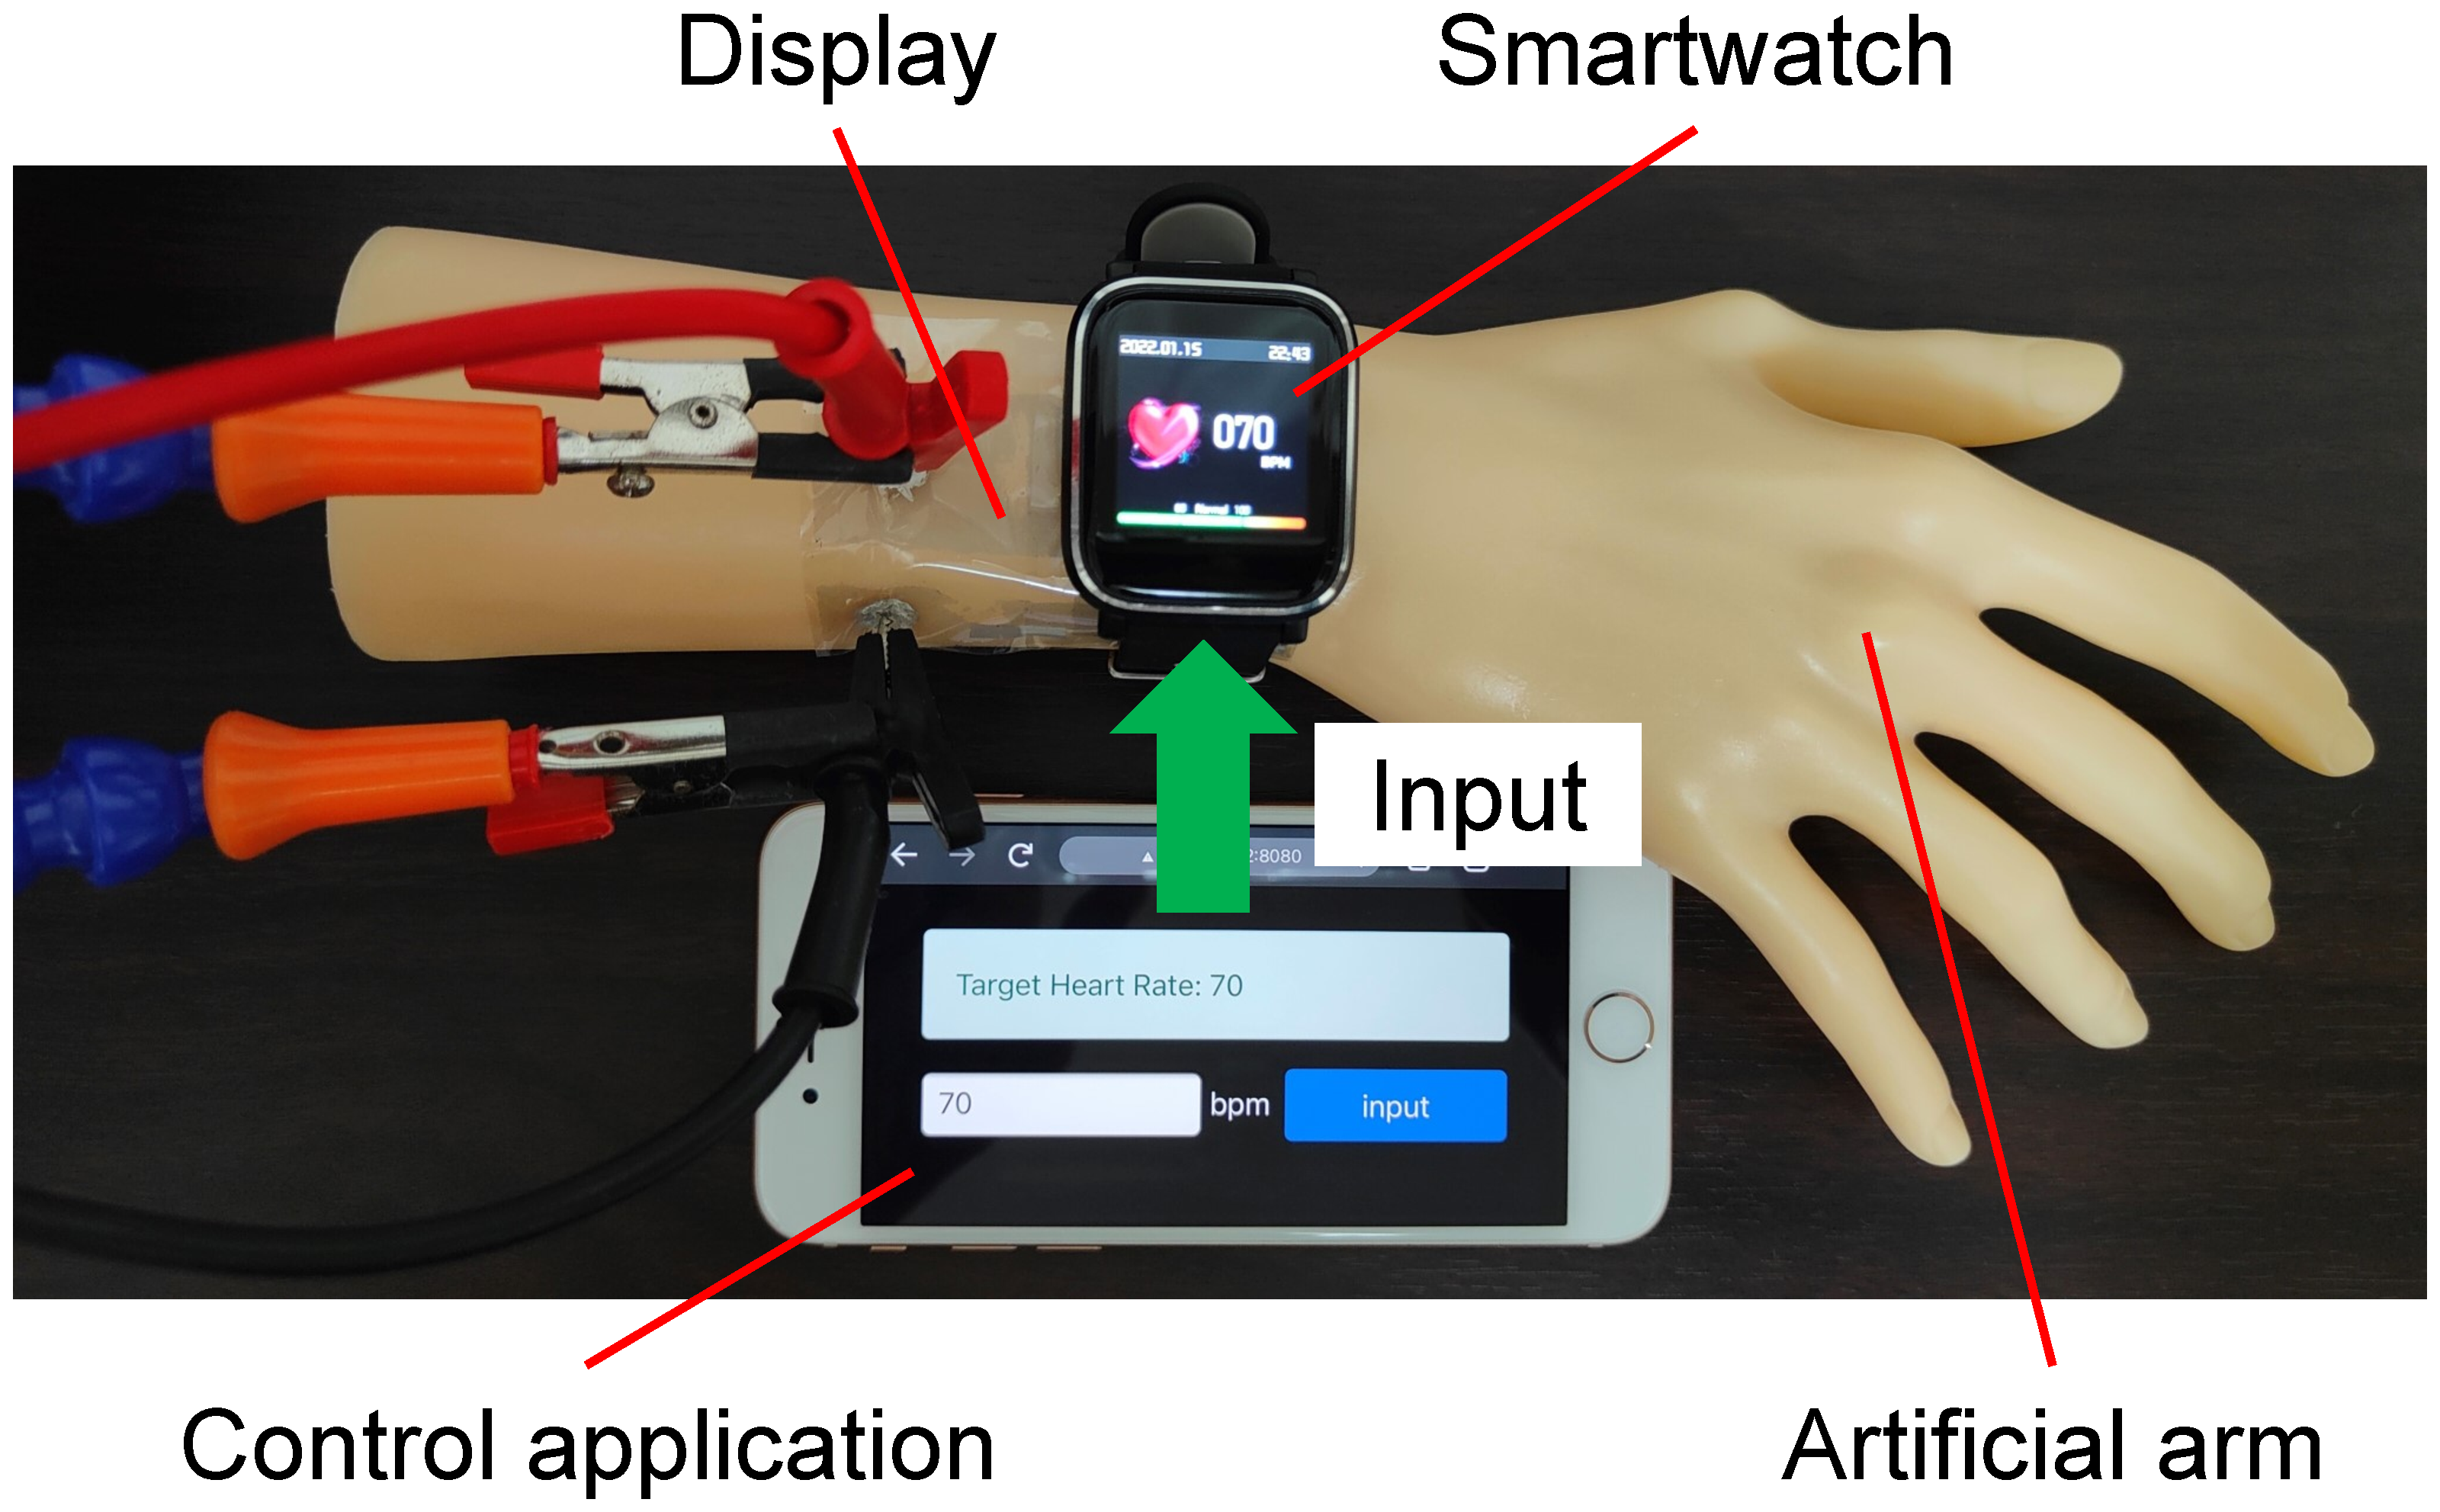
\includegraphics[width=1\linewidth]{figure/system.eps}
  \end{center}
  \caption{システム構成}
  \label{system}
\end{figure}